\documentclass[a4paper]{article}

\usepackage[english]{babel}
\usepackage[utf8x]{inputenc}
\usepackage{amsmath}
\usepackage{graphicx}
\usepackage[colorinlistoftodos]{todonotes}
\usepackage{hyperref}

\newcommand{\ie}{\emph{i.e.}, }

\title{Beacon Follower}
\author{Jakub \v{S}m\'{i}da, Eva Tesa\v{r}ov\'{a}, Jakub Valtar}
\date{}

\begin{document}
\maketitle
\section*{Robot Task}
The task of our robot is to continuously follow a beacon which can change position while the robot is following it. If the distance between the robot and the beacon is sufficiently small, the robot will stop (see Fig.~\ref{fig:beacon}). While following the beacon the robot is avoiding obstacles. Obstacles are represented by a shape made with a different color tape on the floor. The robot uses two motors (connected to wheels) for movement, infrared sensor for localization of the beacon and color sensor for detection of obstacles (see Fig.~\ref{fig:obstacle}).  

\begin{figure}[h]
\centering
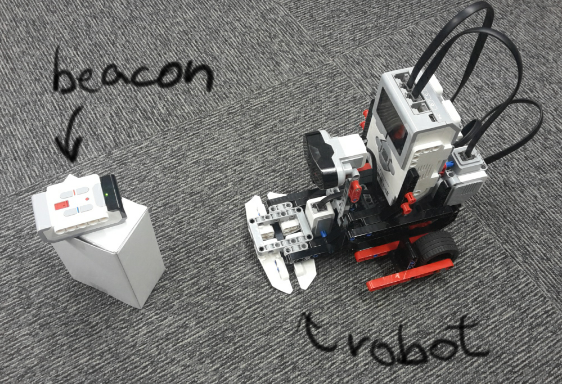
\includegraphics[width=0.7\textwidth]{beacon.png}
\caption{\label{fig:beacon}Beacon follower}
\end{figure}

\begin{figure}[h]
\centering
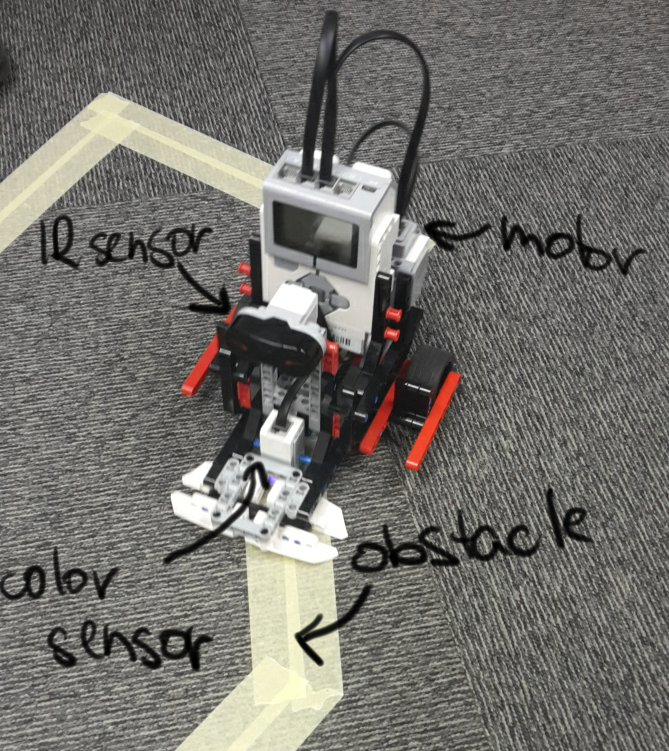
\includegraphics[width=0.7\textwidth]{obstacle.png}
\caption{\label{fig:obstacle}Robot avoiding an obstacle}
\end{figure}

\section*{Robot behavior}
In the beginning, robot waits for a button to be pressed. 

\begin{itemize}
\item By pressing the ENTER button the robot starts to fulfill its task with preset ground and obstacle colors. It starts by turning around until it sees the beacon. Once the beacon is detected, it starts to moving towards it. If it hits an obstacle, it begins to go around it to the left until the way to beacon is free.
\item If the UP button is pressed, robot is waiting to be calibrated by placing it on a ground for reading a ground color and on an obstacle for reading an obstacle color. On each surface, robot moves a little bit to collect more samples. Then it starts to execute the main program, like in the previous case.
\end{itemize}


\section*{Description of the Solution}

\subsection*{Technology}
The robot is built using following components:
\begin{itemize}
\item EV3 Brick
\item EV3 Infrared Sensor
\item EV3 Color Sensor
\item $2\times$ EV3 Large Servo Motor
\end{itemize}

The robot is moving using two wheels, fixed on both sides of the EV3 Brick. To power the wheels we used two EV3 Large Servo Motors. While moving, it uses EV3 Infrared Sensor to detect beacon distance and direction. For obstacle detection the EV3 Color Sensor is used.

\smallskip
We used LeJos 0.9.1 for programming robot's behavior. 

\subsection*{Solution Approach}
We decided to use \textit{behavior trees} to drive robot's behavior (see e.g. \url{http://www.gamasutra.com/blogs/ChrisSimpson/20140717/221339/Behavior_trees_for_AI_How_they_work.php}).

In a shortcut, behavior trees allow us to specify robot's behavior using data (nodes). There are different types of tree nodes (as described below), each fulfilling different task. Some represent conditions, some actions and some are used to combine multiple nodes or change behavior of child node. Program walks through the tree periodically and executes nodes. Nodes run their tasks and return their state as SUCCESS, FAIL or RUNNING. Parent nodes generally return RUNNING while some children are RUNNING. The tree is fulfilled when the root node returns SUCCESS or FAIL. If a node is a leaf, then it is an action which eventually completes or condition which returns its result right away.

\bigskip
\noindent
There are many types of inner nodes, we use following:
\begin{description}
\item[Selector] executes children in order until one of them returns SUCCESS, then it succeeds. If all nodes fail, selector fails too.
\item[Sequence] executes children in order until one of them returns FAIL, then it fails. If all nodes succeed, selector succeeds too.
\item[Invertor] success iff descendant did not success
\item[Failer] always fails
\end{description}

\noindent
Design of implemented behavior tree is depicted in the Fig.~\ref{fig:behaviour_tree}.  

\begin{figure}[h]
\centering
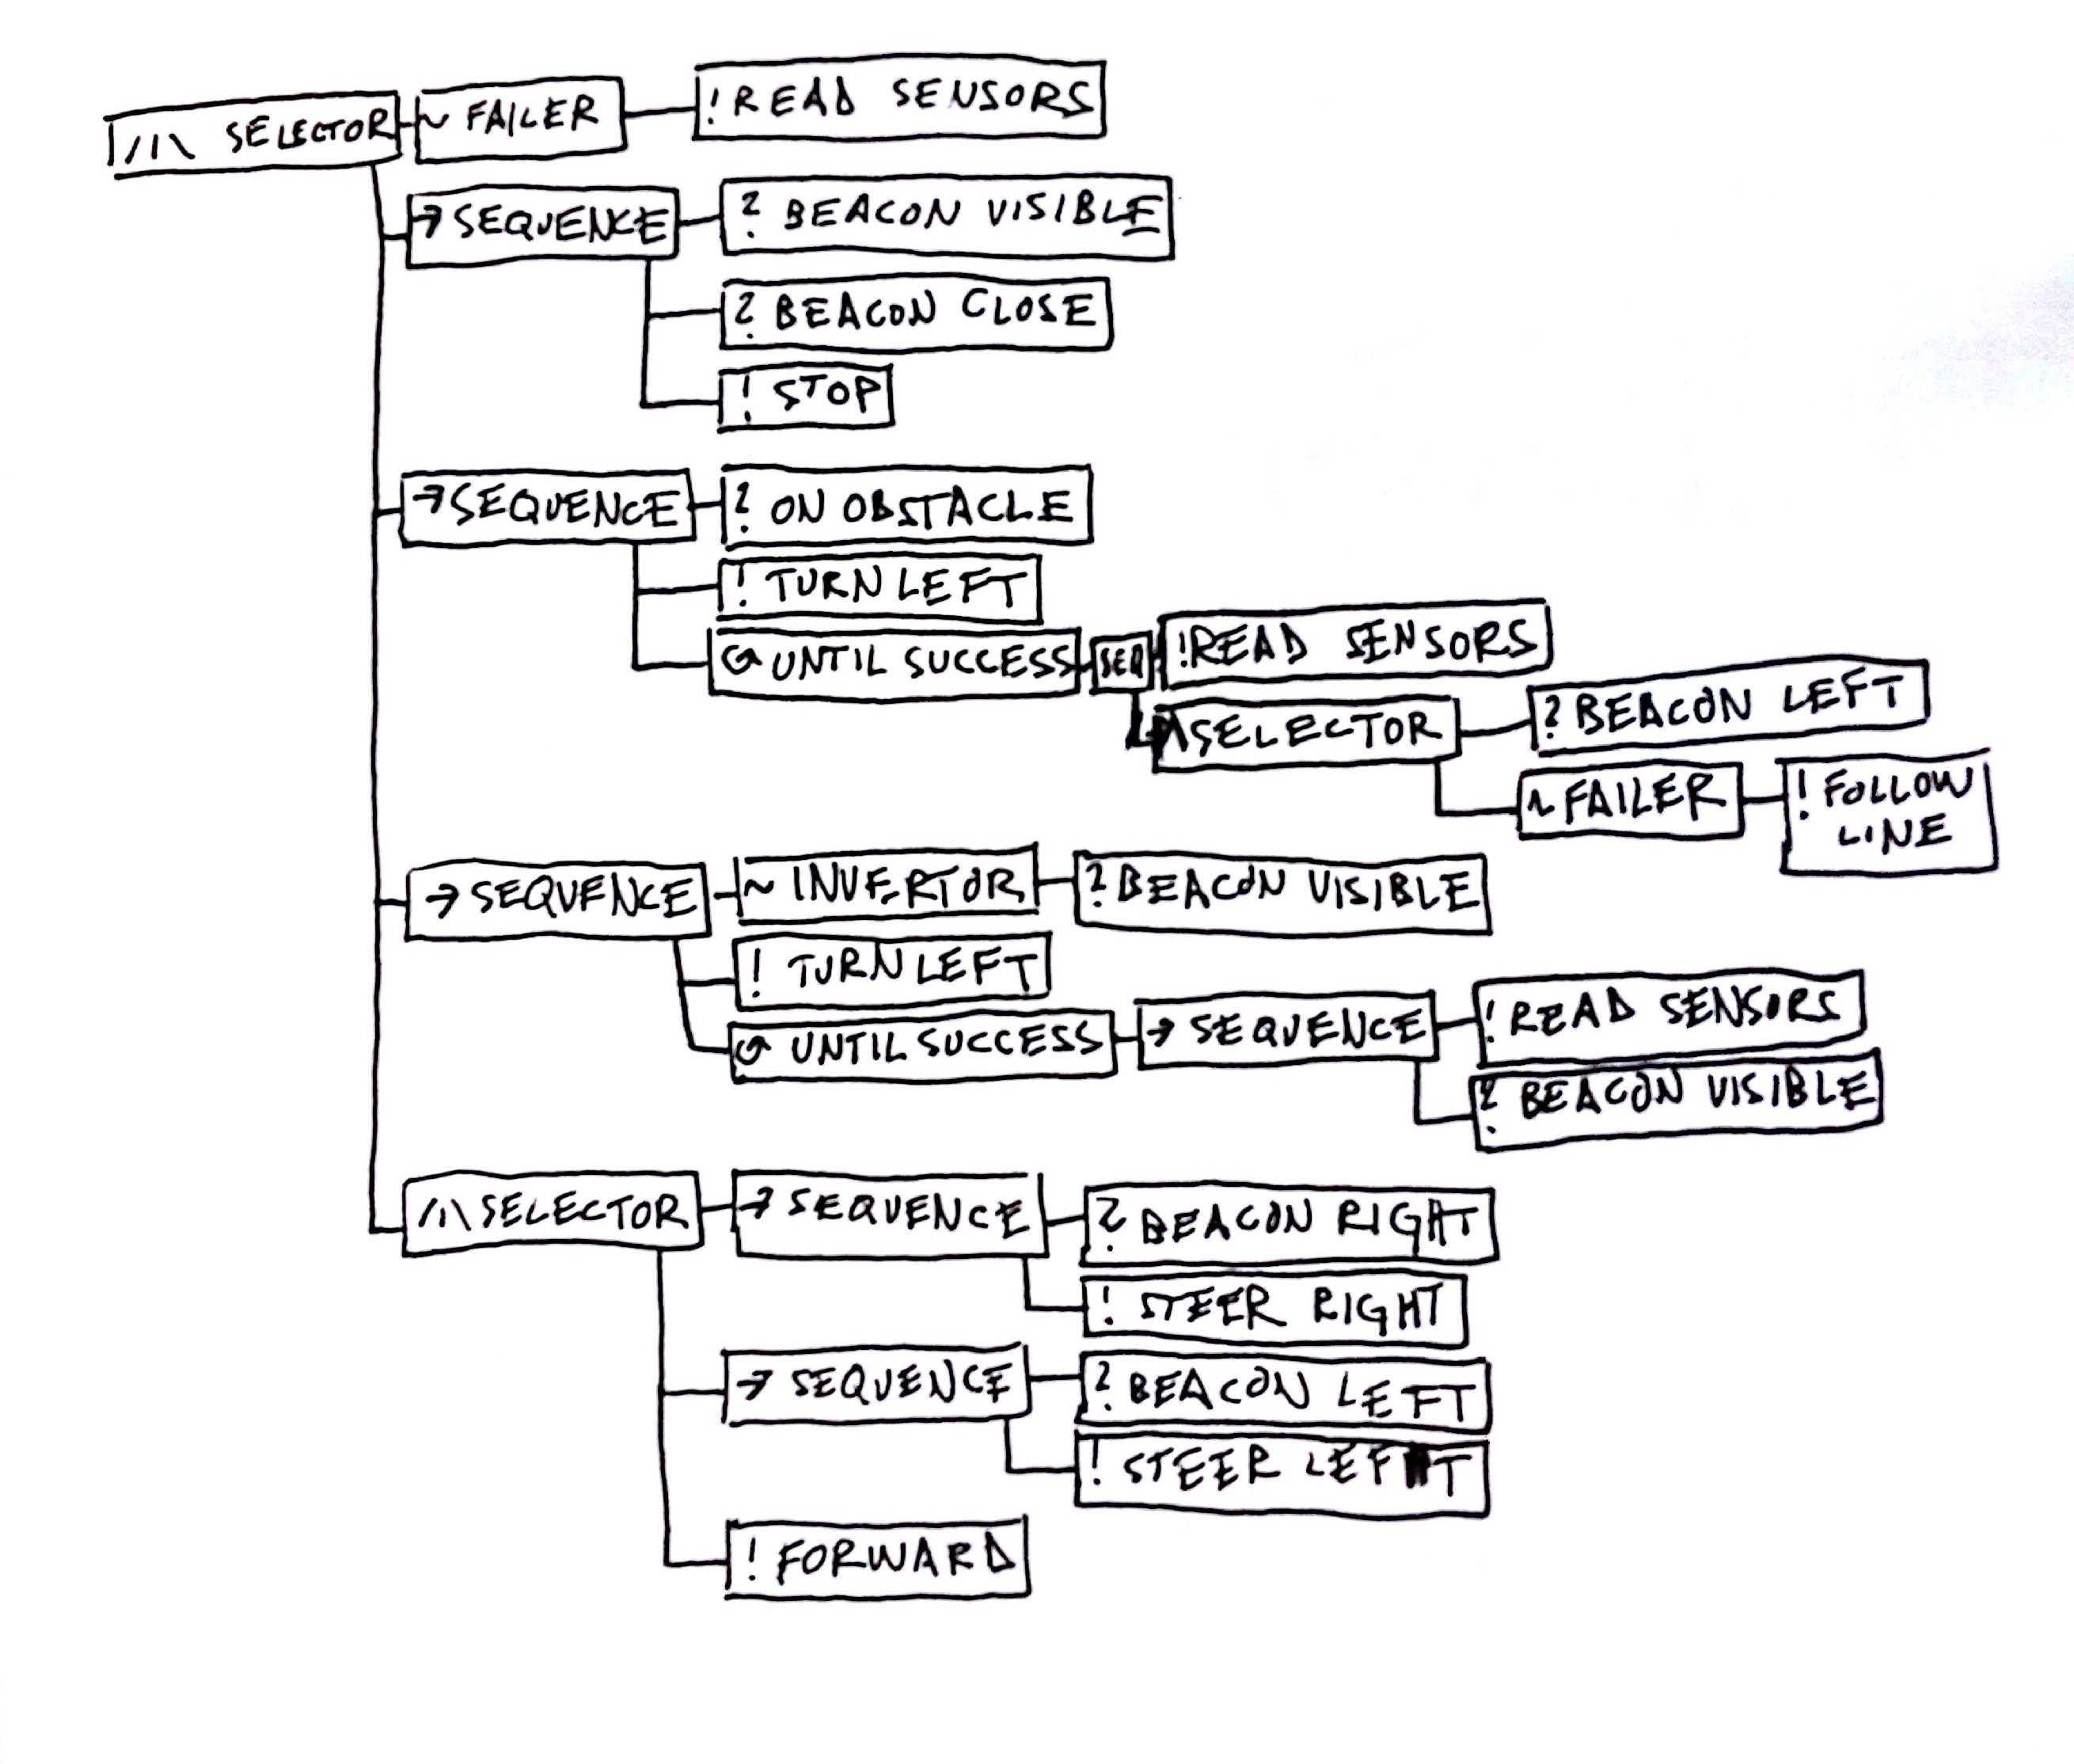
\includegraphics[width=\textwidth]{tree.jpg}
\caption{\label{fig:behaviour_tree}Behaviour tree of the robot}
\end{figure}

\smallskip
Implementation of leafs in the tree is quite straightforward, only complex function is the function \texttt{FollowLine}. The robot knows what is the lightness on the edge of the obstacle and is trying to follow it, \ie the higher is deviation from this value, the more the robot turns to compensate (direction depends on whether last lightness reading is closer to an obstacle lightness, or ground lightness). The turning speed is proportional to the fourth power of the deviation from lightness of the edge. We also adjust forward speed, the more robot has to turn, the lower speed is set, \ie if it follows straight line it goes faster than in curves. 

\subsection*{Implementation}
We used LeJos 0.9.1. to implement robot behavior. Classes \texttt{EV3IRSensor}, \texttt{EV3ColorSensor} are used for communication with sensors and the robot's movement is driven by a \texttt{WheeledChassis} class. 


\subsection*{Concurrency}
Main thread executes the main loop of our program. In each pass, the behavior tree is executed. Action nodes of behavior tree submit tasks to executor, which runs them on a background thread. Nodes return state RUNNING until their tasks on background thread complete, in which case they return either SUCCESS or FAIL (depending on the outcome) and in the next pass the tree executes following nodes. All access to robot's hardware (reading sensors, controlling motors] happens via tasks on the background thread. Main thread keeps executing the tree and checking status of background tasks.

\section*{Complications}
%Meli bychom tam dat komplikace, ale nenapada me, jaky jsme meli -- mozna to, ze kdyz je sensor moc vysoko, tak to davalo spatny data? Komplikace s DifferentialPilot? To jedno vlakno se nam nespoustelo taky, ale vime cim to bylo? Asi taky to, ze se nam beacon odrazi pravdepodobne od sten.
\subsection*{Color sensor} 

We discovered that it is crucial to put the color sensor in the right height from the ground. When the sensor was put too low, robot had only very local information about line edge and its drive while line following was very ``absentminded''. When it was too high, the readings were inaccurate and noise with only a small difference between ground and obstacle.

\subsection*{Beacon signal}
We encountered many times problem with beacon signal when robot suddenly turned around and started to try to follow beacon in the opposite direction than where it actually was. We think that this problem was probably caused by reflection of the signal from the walls and other nearby objects. we didn't manage to solve this problem and we think it would be very difficult to deal with it.

\subsection*{Starvation}
We had to let the main thread sleep for a few milliseconds after each behavior tree traversal to allow background thread to take over and execute submitted tasks. If the background thread is not allowed to run, the main thread keeps getting RUNNING from the affected Action nodes and the program can't move forward.

\section*{Contributions}
\begin{description}
\item[Jakub \v{S}m\'{i}da] hardware designer, implementation of several methods, testing
\item[Eva Tesa\v{r}ov\'{a}] implementation of several methods, project report
\item[Jakub Valtar] main programmer and algorithm designer, project report
\end{description}

\section*{Conclusion}
The robot managed to follow the beacon while avoiding obstacles. Obstacle avoiding was done in a quite smooth manner, however there is still place for improvement. It was sometimes hard for the robot to deal with non-convex obstacles, because it managed to get through the obstacle boundary into the interior and get trapped inside.

\end{document}